\chapter{Introducción}
\label{capitulo1}
\lhead{Capítulo 1. \emph{Introducción}}
% De qué va a tratar el capítulo

La navegación y exploración en áreas de difícil acceso mediante el uso de robots, es una tarea que se ha venido desarrollando en el Grupo de Investigación y Desarrollo en Mecatrónica de la USB  \textit{(GIDM)} desde hace mucho tiempo. Donde una de las aplicaciones mas demandadas, es la tarea de reconstruir un mapa 2D de la superficie mapeada por los robots utilizados. En el presente capitulo se pretende introducir los trabajos previos y avances que se han tenido en el desarrollo de este tipo aplicaciones, específicamente en el \textit{GIDM}, que dieron origen y motivación para la realización del proyecto. Además de postular un serie de problemas que el presente trabajo busca solucionar.

\section{Antecedentes}

En el \textit{GIDM} se han realizado grandes avances en el desarrollo de equipos y plataformas robóticas para actividades de investigación, exploración e inspección de ambientes no estructurados. Usualmente cuando se opera en este tipo de ambientes, en busca de realizar exploraciones mas eficientes y a mayor escala, se emplean vehículos operados remotamente \textit{ROV} (del inglés: Remotely Operated Vehicles) equipados con cámaras de vídeo. O bien, para el caso de aplicaciones subacuáticas también se suelen utilizar vehículos autónomos submarinos \textit{AUV} (del inglés: Automated Underwater Vehicles), mientras que para exploraciones aéreas se hace uso de vehículos aéreos no tripulados UAV (del ingles: Unmanned Aerial Vehicle).

En este sentido, se tienen proyectos como el presentado por \textit{Danilo, D.} \cite{danilo}, cuyo trabajo de grado consistió en el desarrollo en un sistema de operación remota para un robot submarino (\textit{ROV}), con la finalidad de implementarlo en tareas de exploración. Con objetivos similares, \textit{Said, A.} \cite{said} basó su proyecto de grado en la instrumentación y control de un robot cuadricóptero volador(\textit{AUV}). 

Adicional a los proyectos antes mencionados, en el el \textit{GIDM}  se cuenta con un vehículo submarino llamado OpenROV\footnote{ \url{https://www.openrov.com/products/openrov28/}}, el cual es un robot maniobrado remotamente de baja envergadura, diseñado especialmente para operar bajo el agua.

\begin{figure}[H]
	\centering
	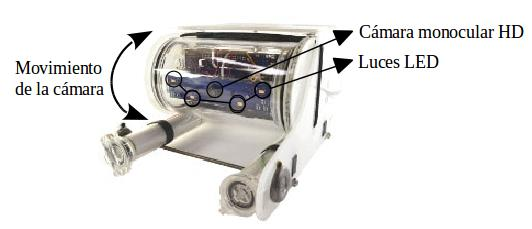
\includegraphics[width=0.7\textwidth]{openrov}
	\caption{Robot móvil OpenROV}
	\label{imagen:openrov}
\end{figure}
Si bien se cuenta con un conjunto de plataformas robóticas adaptadas para tareas de exploración, hasta el momento no se han desarrollados sistemas basados en visión que permitan incluirse en la etapa de navegación y mapeo de dichos vehículos, siendo la presente investigación la primera en abordar la tarea de la reconstrucción del suelo recorrido haciendo uso únicamente de una cámara de vídeo, sensor presente en todas las plataformas robóticas antes mencionados.

\section{Justificación y planteamiento del problema}


Cuando se habla de construir un mosaico 2D, se hace referencia al proceso de recortar y alinear imágenes, de tal forma que puedan ser representadas todas juntas en una sola gran imagen. Es importante considerar que las imágenes para este tipo de aplicaciones son capturadas desde diferentes ubicaciones de la cámara, a diferencia del proceso para elaborar imágenes panorámicas, en las cuales esta ubicación es una constante. Esta característica trae consigo uno de los principales problemas en la construcción de mosaicos, y se debe al efecto paralaje. Este efecto está asociado a la diferencia entre las posiciones aparentes de los objetos, según el punto desde donde se observa.

En la figura \ref{imagen:paralaje} se aprecia un ejemplo ilustrativo de esta definición, en la cual, si nos fijamos en el punto de vista \textbf{A}, se observa la estrella a la izquierda del circulo, mientras que desde le punto \textbf{B} este orden se encuentra invertido. 

\begin{figure}[H]
	\centering
	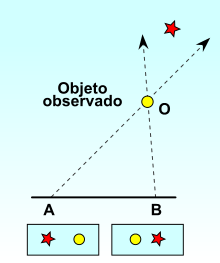
\includegraphics[width=0.4\textwidth]{paralaje1}
	\caption[Efectos en el cambio del punto de vista]{Efectos en el cambio del punto de vista.}
	\label{imagen:paralaje}
\end{figure}

Si bien, este problema afecta en gran medida la construcción del mosaico, no es el único presente, y se intensifican en aplicaciones de mapeo submarino, en las cuales, se evidencian efectos de distorsión de los objetos, absorción y cambios en la dirección de la luz, producto de pequeñas partículas suspendidas en el agua.

\begin{wrapfigure}{r}{0.3\textwidth}
	\begin{center}
		\vspace*{-0.5in}
		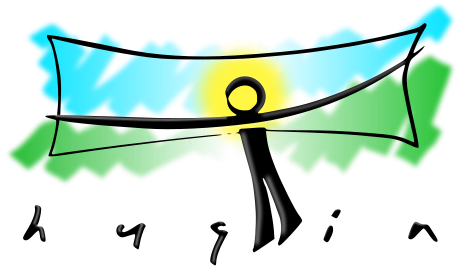
\includegraphics[width=0.3\textwidth]{hugin}
	\end{center}
	\caption{Logo del software Hugin}
\end{wrapfigure}

En el \textit{GIDM} actualmente se utilizan mecanismos manuales para la elaboración de estos mapas, en especifico, se hace uso de \textit{softwares} como Hugin\footnote{\url{hugin.sourceforge.net/}}. Este es un programa de código abierto y gratuito bajo licencia GPL\footnote{ \url{http://www.gnu.org/copyleft/gpl.html}}, el cual esta dedicado a la generación de imágenes panorámicas, incluyendo funciones para el recorte, alineación y corrección de color; además de algoritmos para la optimización de parámetros en la cámara, y corrección de distorsión. Si bien este software esta diseñado para la creación de imágenes panorámicas, permite el uso de varios tipos de proyecciones cartográficas, entre estas la rectangular, proyectando las imágenes sobre un plano recto. 

Esta practica manual, además de limitar el alcance de los sistemas embebidos para el uso en navegación automática, requiere de una inversión de tiempo importante por medio del usuario en el proceso de selección y alineación de imágenes.


Atendiendo a esta necesidad, es necesario contar con un sistema que permita realizar la reconstrucción del suelo con la menor interacción posible del ser humano. Asimismo, con el fin de poder realizar operaciones de mapeo y localización simultanea \textit{SLAM} (del ingles: Simultaneous Localization and Mapping), haciendo uso de las herramientas y robots existentes en el laboratorio, se requiere contar con un sistema basado en visión, que genere de forma automática un mapa 2D de la superficie sobre la que navega o sobrevuela el vehículo remoto, y que logre lidiar de manera efectiva ante los problemas previamente planteados.


\section{Objetivos}

\subsection{Objetivo General}

Analizar e implementar un sistema automatizado que permita la reconstrucción de un mapa en dos dimensiones, del suelo recorrido por robot, aéreo o submarino, a través de la información capturada por una cámara ubicada en su parte inferior.

\subsection{Objetivos Específicos}

\begin{itemize}
	\item Análisis comparativo de métodos vigentes en la reconstrucción de mosaicos 2D, a partir de imágenes y videos de entrada.
	\item Implementación de modulo de pre-procesamiento y corrección de entrada.
	\item Análisis comparativo de métodos de detección y descripción de puntos característicos.
	\item Implementación de módulo de alineación de imágenes mediante la detección de puntos característicos.
	\item Cuantificar el error de proyección y distorsión en los modelos 2D generados.
\end{itemize}

\section{Estructura del trabajo}

Luego de presentar el planteamiento del problema y la descripción del proyecto, la presente investigación se encuentra dividida en 5 capítulos, organizados de la siguiente manera:

En el \textit{\textbf{Capitulo 2}} se presenta una revisión del estado del arte sobre los algoritmos de generación de mosaico, en el cual se exponen los trabajos recientes y avances importantes en esta área de investigación. Al mismo tiempo, se describen los módulos principales que componen este tipo de sistemas. Luego, en base a los algoritmos y técnicas estudiadas se propone un esquema para un sistemas de generación de mosaico. Para finalizar, se presenta la librería de procesamiento de imágenes que se planteó utilizar para la implementación de los algoritmos propuestos.

El \textit{\textbf{Capitulo 3}} inicia una revisión teórica en la cual se describe el funcionamiento de los algoritmos detectores, descriptores y emparejadores de características; y posteriormente se presentan resultados de pruebas comparativas entre los mas usados para este tipo de aplicaciones. 

El módulo encargado de la alineación de imágenes en el mosaico, es descrito en el \textit{\textbf{Capitulo 4}}. Al igual que el capitulo anterior, se presenta una revisión teórica de los conceptos necesarios para su implementación. Luego, se introduce el modelo de sub mosaicos, y la implementación de un conjunto de correcciones geométricas sobre este nuevo modelo. Finalmente se muestran los resultados de los algoritmos aplicados en esta sección, seguidos de sus respectivos análisis.

En el \textit{\textbf{Capitulo 5}} se describe el modulo final del sistema, en donde se explica el funcionamiento de los algoritmos que corrigen visualmente el mosaico final. De igual forma se muestran los resultados de su implementación, seguidos de una conclusión final sobre estos.

Finalmente, en el \textit{\textbf{Capitulo 6}} se presentan las conclusiones finales, además de propuestas sobre recomendaciones y posibles implementaciones que pueden aportar mejoras y/o permitir la continuación del proyecto aquí planteado.